\documentclass[a4paper,12pt]{article}

% Pakiety
\usepackage[utf8]{inputenc}
\usepackage[T1]{fontenc}
\usepackage[polish]{babel}
\usepackage{geometry}
\usepackage{graphicx}
\usepackage{amsmath, amssymb}
\usepackage{float}
\usepackage{listings}
\usepackage{xcolor}
\usepackage{hyperref}
\usepackage{booktabs}

\geometry{margin=2.5cm}

\lstset{
    language=Matlab,
    basicstyle=\ttfamily\small,
    keywordstyle=\color{blue},
    stringstyle=\color{red},
    commentstyle=\color{green!60!black},
    numbers=left,
    numberstyle=\tiny,
    stepnumber=1,
    numbersep=5pt,
    frame=single,
    breaklines=true
}

\title{\textbf{Projekt TAP}}
\author{
Krystian Czechowicz \\
Adam Makowski \\
Łukasz Nowaczyński
}
\date{\today}

\begin{document}

\begin{titlepage}
    \centering
    {\Large Politechnika Warszawska\par}
    \vspace{0.3cm}
    {\large Wydział Elektroniki i Technik Informacyjnych \par}
    \vspace{2cm}
    {\Huge \textbf{Projekt TAP -- sprawozdanie 1} \par}
    \vspace{0.5cm}
    {\Large Techniki Automatyzacji Procesów \par}
    \vspace{2cm}
    \textbf{Autorzy:} \par
    \vspace{0.5cm}
    \begin{tabular}{c}
        Krystian Czechowicz \\
        Adam Makowski \\
        Łukasz Nowaczyński
    \end{tabular}
    \vfill
    \vspace{1cm}
    \textbf{Data:} \par
    \today
\end{titlepage}

\tableofcontents
\newpage

% ==============================================================
\section{Opis obiektu}
% ==============================================================

Przedmiotem projektu jest reaktor przepływowy z~mieszadłem (CSTR), w~którym zachodzi egzotermiczna reakcja $A \rightarrow B$. Reaktor jest chłodzony płaszczem wodnym.

Dynamika obiektu opisana jest układem dwóch równań różniczkowych:
\begin{align}
V \frac{dC_A}{dt} &= F_{in} \cdot C_{Ain} - F \cdot C_A - V \cdot k_0 \cdot e^{-\frac{E}{RT}} \cdot C_A \label{eq:ca}\\[6pt]
V \rho c_p \frac{dT}{dt} &= F_{in} \rho c_p T_{in} - F \rho c_p T + V h k_0 e^{-\frac{E}{RT}} C_A - \frac{a \cdot F_C^{b+1}}{F_C + \frac{a \cdot F_C^{b}}{2 \rho_c c_{pc}}} (T - T_{Cin}) \label{eq:T}
\end{align}

\begin{table}[H]
\centering
\begin{tabular}{lll}
\toprule
\textbf{Stała} & \textbf{Wartość} & \textbf{Jednostka} \\
\midrule
$\rho = \rho_c$ & $10^6$ & g/m$^3$ \\
$c_p = c_{pc}$ & 1 & cal/(g$\cdot$K) \\
$k_0$ & $10^{10}$ & 1/min \\
$E/R$ & 8330{,}1 & K \\
$h$ & $130 \cdot 10^6$ & cal/kmol \\
$a$ & $1{,}678 \cdot 10^6$ & cal/(K$\cdot$m$^3$) \\
$b$ & 0{,}5 & -- \\
\bottomrule
\end{tabular}
\caption{Stałe modelu}
\end{table}

\begin{table}[H]
\centering
\begin{tabular}{lll}
\toprule
\textbf{Zmienna} & \textbf{Wartość} & \textbf{Rola} \\
\midrule
$V$ & 1 m$^3$ & objętość reaktora \\
$F_{in} = F$ & 1 m$^3$/min & przepływ \\
$C_{Ain,0}$ & 2 kmol/m$^3$ & sterowanie \\
$F_{C,0}$ & 15 m$^3$/min & sterowanie \\
$T_{in,0}$ & 323 K & zakłócenie \\
$T_{Cin,0}$ & 365 K & zakłócenie \\
$C_{A,0}$ & 0{,}26 kmol/m$^3$ & wyjście \\
$T_0$ & 393{,}9 K & wyjście \\
\bottomrule
\end{tabular}
\caption{Punkt pracy}
\end{table}

% ==============================================================
\section{Symulacja modelu nieliniowego (punkt 1)}
% ==============================================================

\subsection{Postać równań do symulacji}

Po podzieleniu równań (\ref{eq:ca}) i~(\ref{eq:T}) przez odpowiednie stałe i~wprowadzeniu oznaczeń pomocniczych:
\[
\begin{aligned}
p_{11} &= \frac{F_{in}}{V} &\quad p_{12} &= -\frac{F}{V} \\
p_{13} &= -k_0               &\quad p_{14} &= -\frac{E}{R}  \\
p_{21} &= \frac{F_{in}}{V}             &\quad p_{22} &= -\frac{F}{V}  \\
p_{23} &= \frac{hk_0}{\rho c_p}            &\quad p_{24} &= -\frac{E}{R}  \\
p_{25} &= \frac{V\rho c_p}{a}            &\quad p_{26} &= \frac{V}{2}
\end{aligned}
\]

otrzymujemy układ w~postaci Cauchy'ego:
\begin{align}
\frac{dC_A}{dt} &= p_{11}C_{Ain} + p_{12}C_A + p_{13}e^{\frac{p_{14}}{T}}C_A \\[6pt]
\frac{dT}{dt} &= p_{21}T_{in} + p_{22}T+p_{23}e^{\frac{p_{24}}{T}}C_A+\frac{F_C}{p_{25}F_C^{1-b}+p_{26}}(T-T_{Cin})
\end{align}

Model zaimplementowano w~MATLABie z~wykorzystaniem solvera \texttt{ode15s}. Przeprowadzono symulację w~punkcie pracy oraz odpowiedzi na skoki poszczególnych wejść.

\subsection{Wyniki symulacji}

\begin{figure}[H]
    \centering
    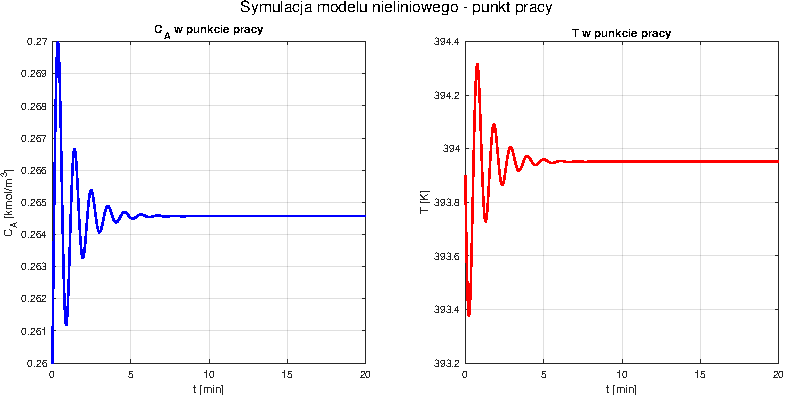
\includegraphics[width=0.95\textwidth]{wykresy/model_punkt_pracy.pdf}
    \caption{Symulacja modelu nieliniowego w~punkcie pracy}
    \label{fig:nl_pp}
\end{figure}

W~punkcie pracy obserwujemy niewielkie tłumione oscylacje. Wynika to z~faktu, że podany punkt pracy ($C_{A,0} = 0{,}26$) jest wartością zaokrągloną -- dokładna równowaga wynosi $C_{A,0} \approx 0{,}2656$.

\begin{figure}[H]
    \centering
    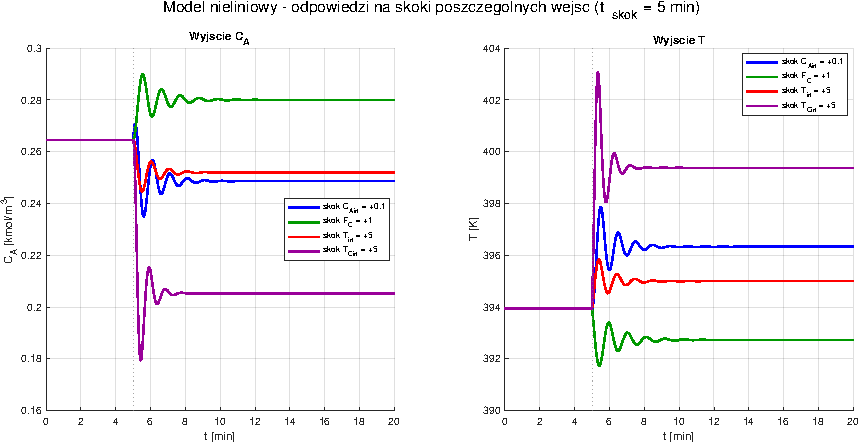
\includegraphics[width=0.95\textwidth]{wykresy/model_odpowiedzi_skokowe.pdf}
    \caption{Odpowiedzi modelu nieliniowego na skoki poszczególnych wejść}
    \label{fig:nl_skoki}
\end{figure}

Na rysunku \ref{fig:nl_skoki} przedstawiono odpowiedzi na 4 scenariusze skokowe (po jednym wejściu zmienianym naraz). Skok następuje w~chwili $t = 5$~min. Widać, że każde wejście wpływa na oba wyjścia, a~system wykazuje oscylacyjny charakter odpowiedzi.

% ==============================================================
\section{Linearyzacja modelu (punkt 1a)}
% ==============================================================

\subsection{Metoda linearyzacji}

Linearyzacja polega na rozwinięciu nieliniowych członów w~szereg Taylora wokół punktu pracy i~odrzuceniu wyrazów wyższych rzędów.

Nieliniowości występujące w~równaniach:
\begin{align}
 p_{13}e^{\frac{p_{14}}{T}}C_A &\approx  p_{13}e^{\frac{p_{14}}{T_0}}C_{A0} + p_{13}e^{\frac{p_{14}}{T_0}}(C_A-C_{A0}) + \frac{-p_{14}}{T_0^2}p_{13}C_{A0}e^{\frac{p_{14}}{T_0}}(T-T_0)\\[6pt]
 p_{23}e^{\frac{p_{24}}{T}}C_A &\approx  p_{23}e^{\frac{p_{24}}{T_0}}C_{A0} + p_{23}e^{\frac{p_{24}}{T_0}}(C_A-C_{A0}) + \frac{-p_{24}}{T_0^2}p_{23}C_{A0}e^{\frac{p_{24}}{T_0}}(T-T_0)\\[6pt]
 \frac{F_C}{p_{25}F_C^{1-b}+p_{26}}T &\approx  \frac{F_{C0}}{p_{25}F_{C0}^{1-b}+p_{26}}T_0 + \frac{F_{C0}}{p_{25}F_{C0}^{1-b}+p_{26}}(T-T_0) \nonumber \\
 &+ T_0\frac{p_{25}F_{C0}^{1-b}+p_{26} - (1-b)F_{C0}p_{25}F_{C0}^{-b}}{(p_{25}F_{C0}^{1-b}+p_{26})^2}(F_C-F_{C0})\\[6pt]
  \frac{F_C}{p_{25}F_C^{1-b}+p_{26}}T_{Cin} &\approx  \frac{F_{C0}}{p_{25}F_{C0}^{1-b}+p_{26}}T_{Cin0} + \frac{F_{C0}}{p_{25}F_{C0}^{1-b}+p_{26}}(T_{Cin}-T_{Cin0})\nonumber \\
  &+ T_{Cin0}\frac{p_{25}F_{C0}^{1-b}+p_{26} - (1-b)F_{C0}p_{25}F_{C0}^{-b}}{(p_{25}F_{C0}^{1-b}+p_{26})^2}(F_C-F_{C0})
\end{align}

\subsection{Model w~przestrzeni stanów}

Zlinearyzowany model zapisujemy w~postaci:
\begin{equation}
    \dot x = Ax + Bu + Cz + D
\end{equation}

gdzie:
\begin{equation}
    x = \begin{bmatrix} C_A\\ T \end{bmatrix}, \quad
    u = \begin{bmatrix} C_{Ain}\\ F_C \end{bmatrix}, \quad
    z = \begin{bmatrix} T_{in} \\ T_{Cin} \end{bmatrix}
\end{equation}

Macierze Jakobianów:
\begin{align}
    A &= \begin{bmatrix}
        p_{12}+p_{13}e^{\frac{p_{14}}{T_0}} &  \frac{-p_{14}}{T_0^2}p_{13}C_{A0}e^{\frac{p_{14}}{T_0}}\\[8pt]
        p_{23}e^{\frac{p_{24}}{T_0}} & p_{22}+ \frac{-p_{24}}{T_0^2}p_{23}C_{A0}e^{\frac{p_{24}}{T_0}}+\frac{F_{C0}}{p_{25}F_{C0}^{1-b}+p_{26}}
    \end{bmatrix}\\[10pt]
    B &= \begin{bmatrix}
        p_{11} & 0 \\[8pt]
        0 & (T_{0}-T_{Cin0})\frac{p_{25}F_{C0}^{1-b}+p_{26} - (1-b)F_{C0}p_{25}F_{C0}^{-b}}{(p_{25}F_{C0}^{1-b}+p_{26})^2}
    \end{bmatrix} \\[10pt]
    C &= \begin{bmatrix}
        0 & 0 \\[8pt]
        p_{21} & \frac{-F_{C0}}{p_{25}F_{C0}^{1-b}+p_{26}}
    \end{bmatrix}
\end{align}

Macierz wyjść: $E = I_{2\times 2}$, $F = G = 0$, $H = 0$.

Wartości własne macierzy $A$ są zespolone z~ujemną częścią rzeczywistą, co potwierdza stabilność układu oraz oscylacyjny charakter odpowiedzi.

\subsection{Transmitancje ciągłe}

Traktując $D$ jako wyrażenie od wejścia stałego $w(t) = 1$, przekształcamy do dziedziny Laplace'a:
\begin{equation}
    Y(s) = G_u(s) U(s) + G_z(s) Z(s) + G_d(s) W(s) + Y(0)
\end{equation}

gdzie:
\begin{align}
    G_u(s) &= (sI-A)^{-1}B \\
    G_z(s) &= (sI-A)^{-1}C \\
    G_d(s) &= (sI-A)^{-1}D
\end{align}

Transmitancje mają wspólny mianownik:
\begin{equation}
    w(s) = s^2 - \text{tr}(A) \cdot s + \det(A)
\end{equation}

Konkretne wartości współczynników obliczono numerycznie w~MATLABie za pomocą funkcji \texttt{tf(ss(A,B,C,D))}.

\subsection{Wyniki -- odpowiedzi modelu liniowego}

\begin{figure}[H]
    \centering
    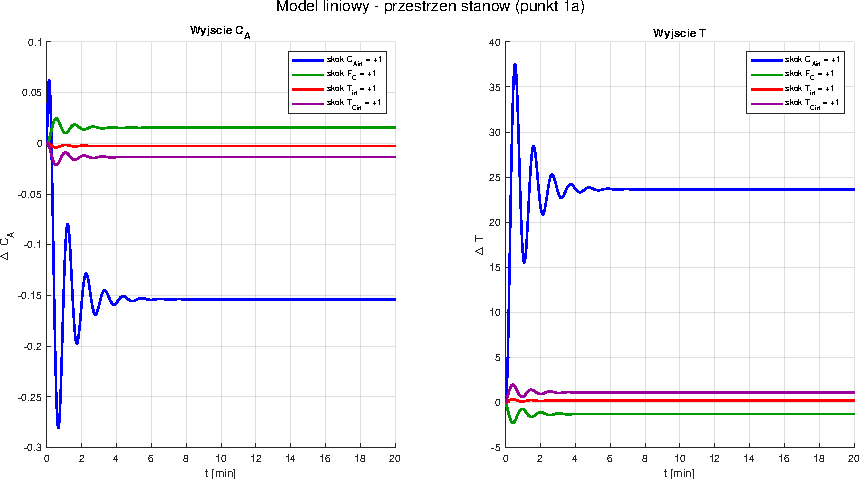
\includegraphics[width=0.95\textwidth]{wykresy/1a_przestrzen_stanow.pdf}
    \caption{Odpowiedzi skokowe modelu liniowego -- przestrzeń stanów (lsim)}
    \label{fig:1a_ss}
\end{figure}

\begin{figure}[H]
    \centering
    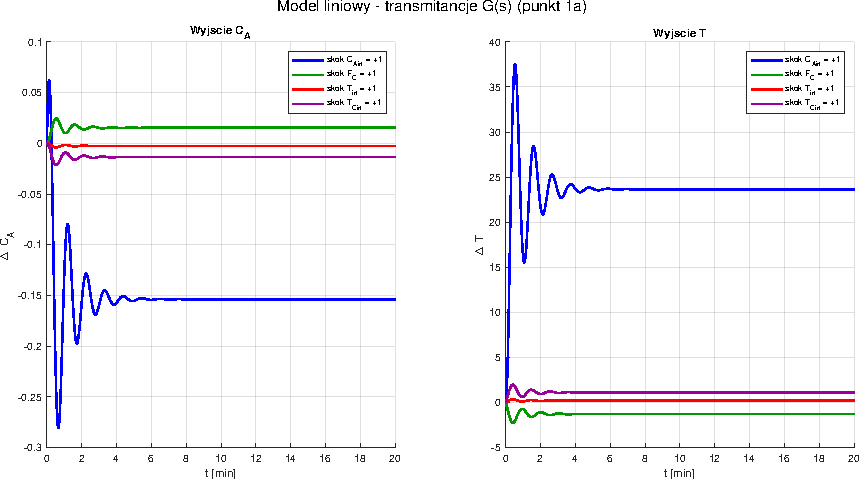
\includegraphics[width=0.95\textwidth]{wykresy/1a_transmitancje.pdf}
    \caption{Odpowiedzi skokowe modelu liniowego -- transmitancje $G(s)$}
    \label{fig:1a_tf}
\end{figure}

Rysunki \ref{fig:1a_ss} i~\ref{fig:1a_tf} przedstawiają odpowiedzi na skoki jednostkowe każdego z~4 wejść. Obie reprezentacje (przestrzeń stanów i~transmitancje) dają identyczne przebiegi, co potwierdza poprawność obliczeń.

% ==============================================================
\section{Porównanie modeli liniowego i~nieliniowego (punkt 1b)}
% ==============================================================

W~celu oceny jakości przybliżenia liniowego przeprowadzono osobne symulacje skokowe dla każdego wejścia przy dwóch amplitudach (małej i~dużej, zarówno dodatniej jak i~ujemnej). Na każdym wykresie porównano odpowiedź modelu nieliniowego (linia ciągła niebieska) z~modelem liniowym (linia przerywana czerwona). Skok następuje w~chwili $t = 5$ min.

% --- CAin ---

\begin{figure}[H]
    \centering
    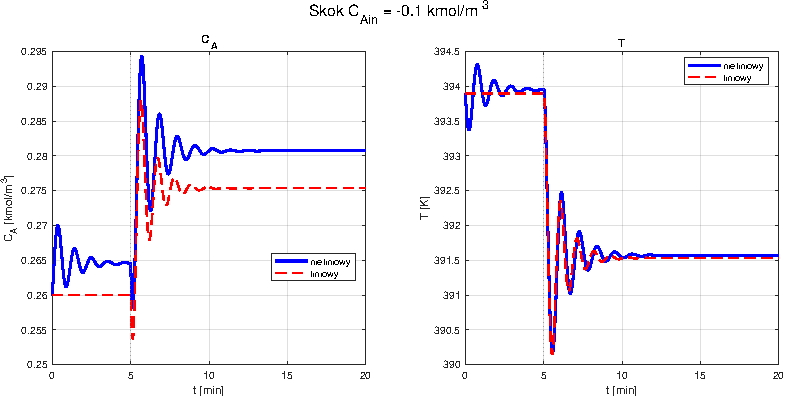
\includegraphics[width=0.95\textwidth]{wykresy/1b_CAin_m0.1.pdf}
    \caption{Skok $\Delta C_{Ain} = -0{,}1$ kmol/m$^3$}
    \label{fig:1b_cain_m01}
\end{figure}

\begin{figure}[H]
    \centering
    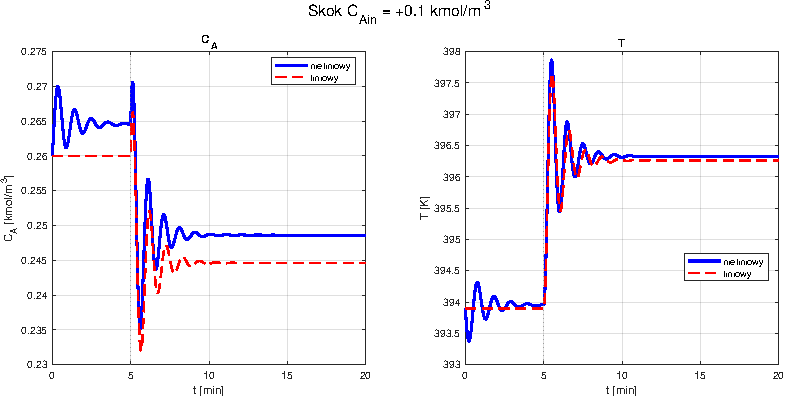
\includegraphics[width=0.95\textwidth]{wykresy/1b_CAin_p0.1.pdf}
    \caption{Skok $\Delta C_{Ain} = +0{,}1$ kmol/m$^3$}
    \label{fig:1b_cain_p01}
\end{figure}

\begin{figure}[H]
    \centering
    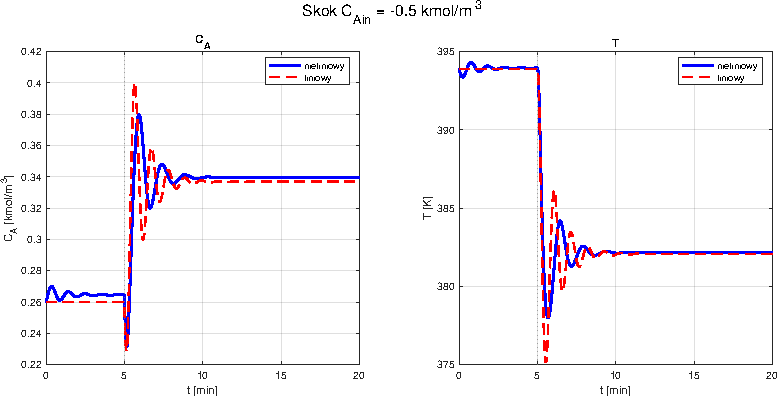
\includegraphics[width=0.95\textwidth]{wykresy/1b_CAin_m0.5.pdf}
    \caption{Skok $\Delta C_{Ain} = -0{,}5$ kmol/m$^3$}
    \label{fig:1b_cain_m05}
\end{figure}

\begin{figure}[H]
    \centering
    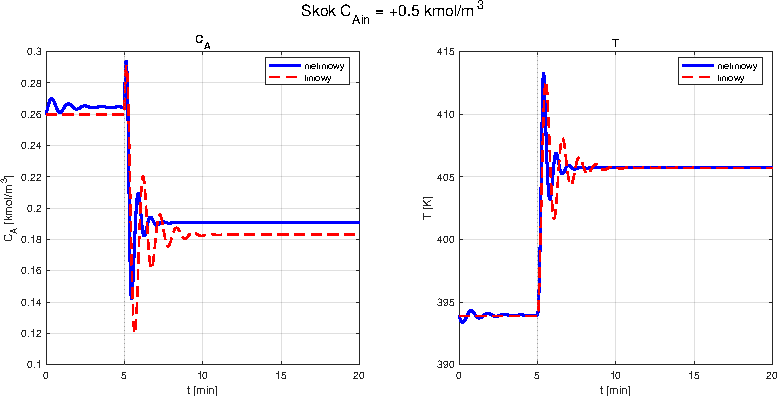
\includegraphics[width=0.95\textwidth]{wykresy/1b_CAin_p0.5.pdf}
    \caption{Skok $\Delta C_{Ain} = +0{,}5$ kmol/m$^3$}
    \label{fig:1b_cain_p05}
\end{figure}

% --- FC ---

\begin{figure}[H]
    \centering
    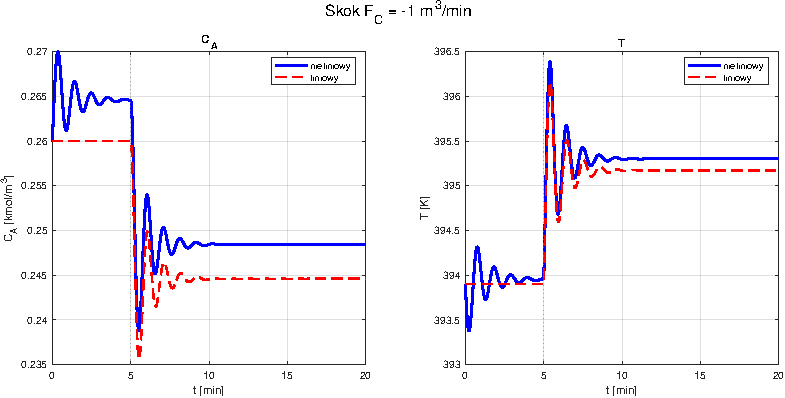
\includegraphics[width=0.95\textwidth]{wykresy/1b_FC_m1.pdf}
    \caption{Skok $\Delta F_C = -1$ m$^3$/min}
    \label{fig:1b_fc_m1}
\end{figure}

\begin{figure}[H]
    \centering
    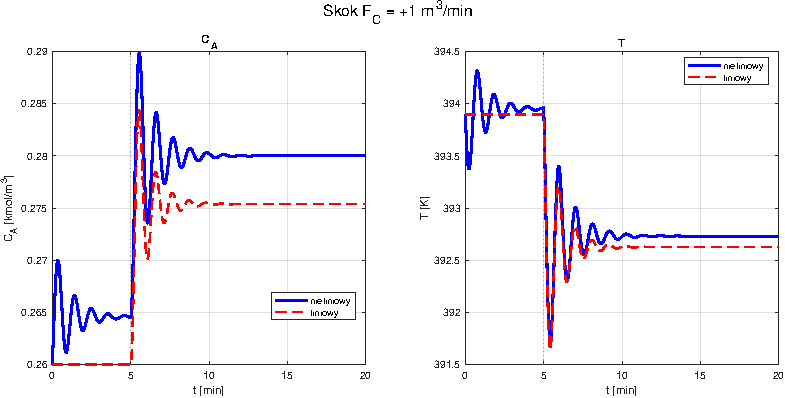
\includegraphics[width=0.95\textwidth]{wykresy/1b_FC_p1.pdf}
    \caption{Skok $\Delta F_C = +1$ m$^3$/min}
    \label{fig:1b_fc_p1}
\end{figure}

\begin{figure}[H]
    \centering
    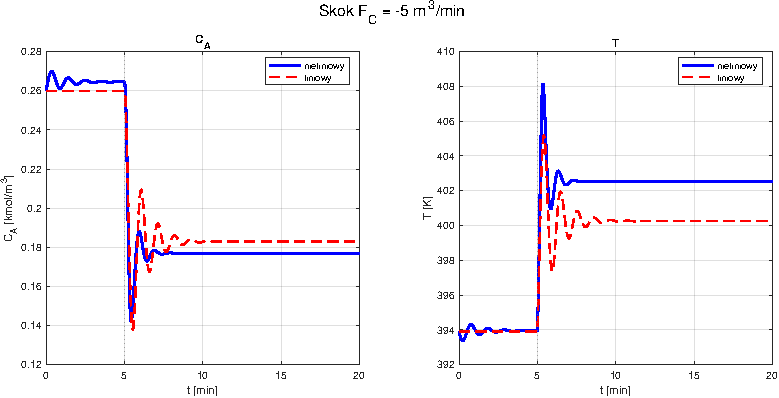
\includegraphics[width=0.95\textwidth]{wykresy/1b_FC_m5.pdf}
    \caption{Skok $\Delta F_C = -5$ m$^3$/min}
    \label{fig:1b_fc_m5}
\end{figure}

\begin{figure}[H]
    \centering
    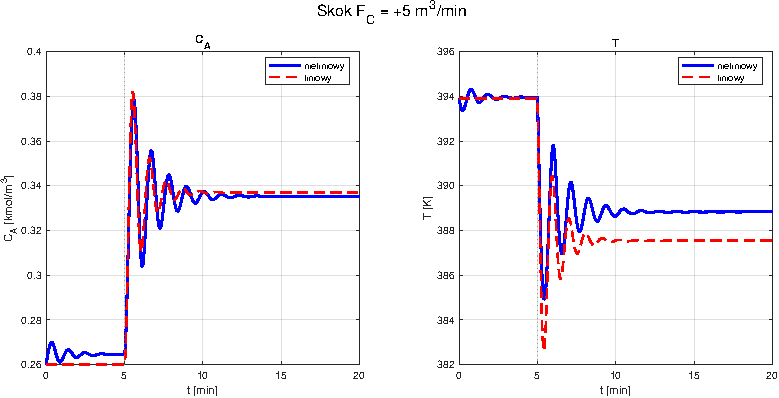
\includegraphics[width=0.95\textwidth]{wykresy/1b_FC_p5.pdf}
    \caption{Skok $\Delta F_C = +5$ m$^3$/min}
    \label{fig:1b_fc_p5}
\end{figure}

% --- Tin ---

\begin{figure}[H]
    \centering
    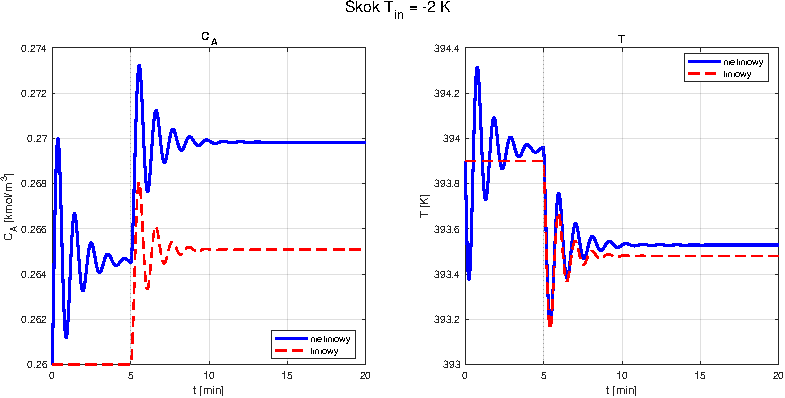
\includegraphics[width=0.95\textwidth]{wykresy/1b_Tin_m2.pdf}
    \caption{Skok $\Delta T_{in} = -2$ K}
    \label{fig:1b_tin_m2}
\end{figure}

\begin{figure}[H]
    \centering
    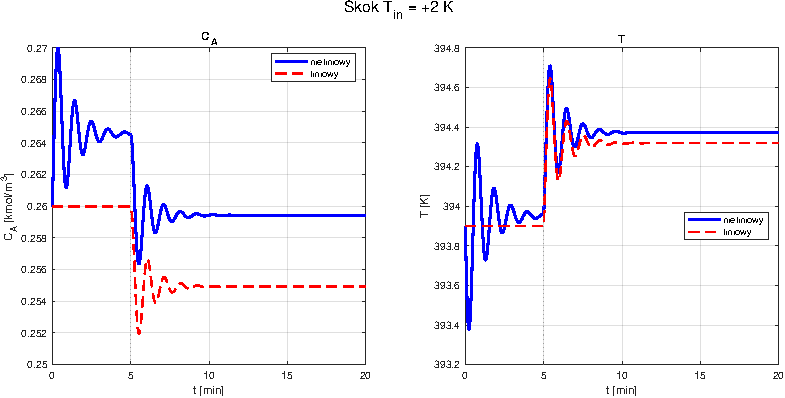
\includegraphics[width=0.95\textwidth]{wykresy/1b_Tin_p2.pdf}
    \caption{Skok $\Delta T_{in} = +2$ K}
    \label{fig:1b_tin_p2}
\end{figure}

\begin{figure}[H]
    \centering
    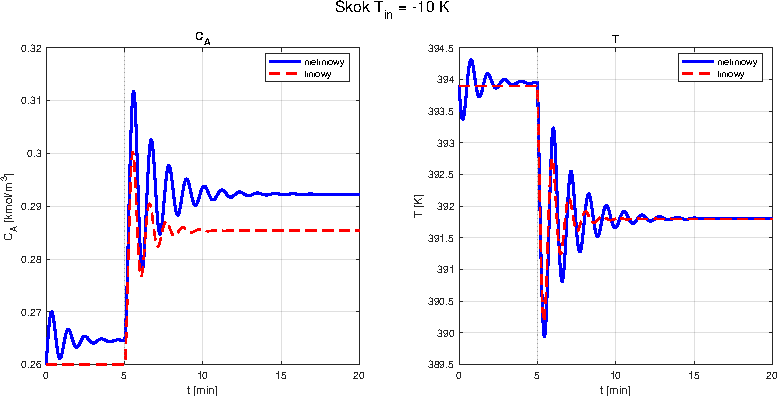
\includegraphics[width=0.95\textwidth]{wykresy/1b_Tin_m10.pdf}
    \caption{Skok $\Delta T_{in} = -10$ K}
    \label{fig:1b_tin_m10}
\end{figure}

\begin{figure}[H]
    \centering
    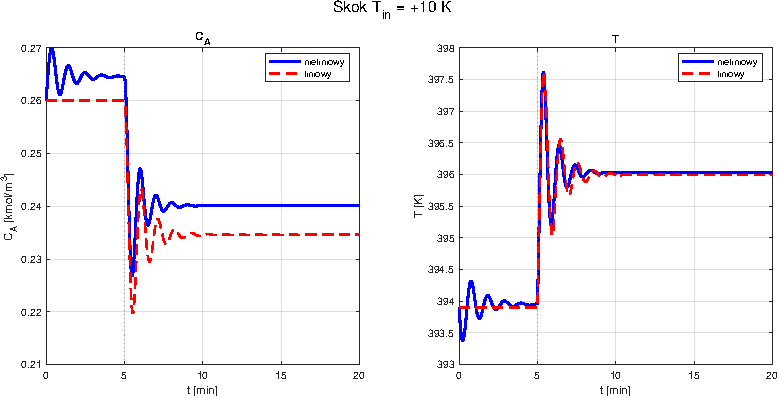
\includegraphics[width=0.95\textwidth]{wykresy/1b_Tin_p10.pdf}
    \caption{Skok $\Delta T_{in} = +10$ K}
    \label{fig:1b_tin_p10}
\end{figure}

% --- TCin ---

\begin{figure}[H]
    \centering
    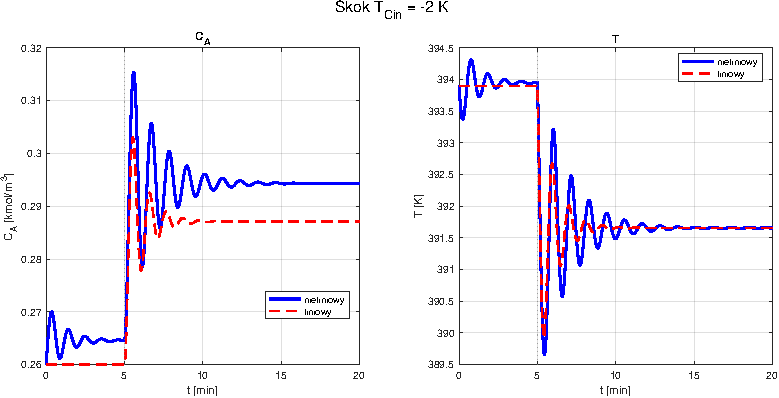
\includegraphics[width=0.95\textwidth]{wykresy/1b_TCin_m2.pdf}
    \caption{Skok $\Delta T_{Cin} = -2$ K}
    \label{fig:1b_tcin_m2}
\end{figure}

\begin{figure}[H]
    \centering
    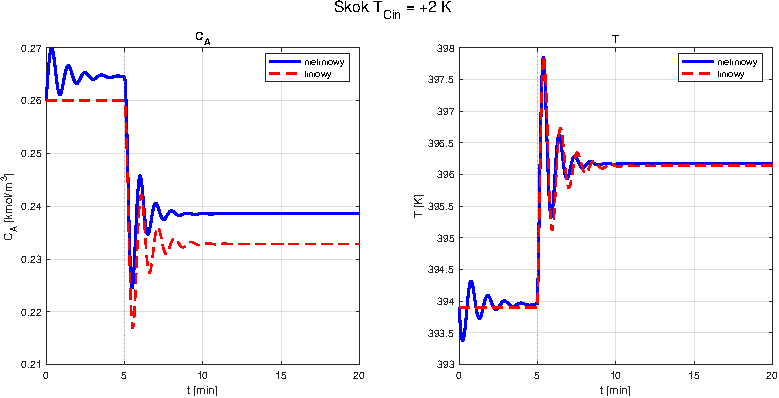
\includegraphics[width=0.95\textwidth]{wykresy/1b_TCin_p2.pdf}
    \caption{Skok $\Delta T_{Cin} = +2$ K}
    \label{fig:1b_tcin_p2}
\end{figure}

\begin{figure}[H]
    \centering
    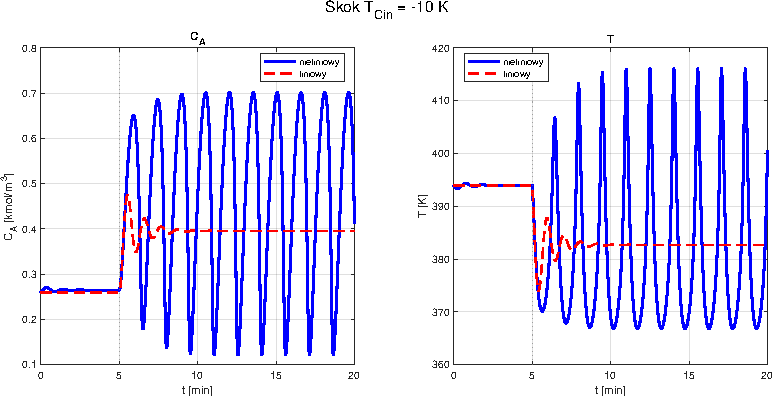
\includegraphics[width=0.95\textwidth]{wykresy/1b_TCin_m10.pdf}
    \caption{Skok $\Delta T_{Cin} = -10$ K}
    \label{fig:1b_tcin_m10}
\end{figure}

\begin{figure}[H]
    \centering
    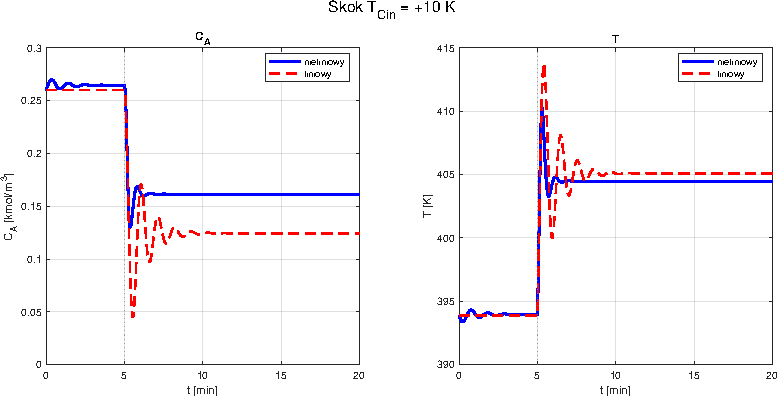
\includegraphics[width=0.95\textwidth]{wykresy/1b_TCin_p10.pdf}
    \caption{Skok $\Delta T_{Cin} = +10$ K}
    \label{fig:1b_tcin_p10}
\end{figure}

\subsection{Obserwacje}

\begin{enumerate}
    \item Dla małych skoków ($\Delta C_{Ain} = \pm 0{,}1$, $\Delta F_C = \pm 1$, $\Delta T_{in} = \pm 2$, $\Delta T_{Cin} = \pm 2$) odpowiedzi obu modeli praktycznie się pokrywają -- model liniowy dobrze przybliża nieliniowy w~otoczeniu punktu pracy.
    \item Ze wzrostem amplitudy różnice rosną, szczególnie w~temperaturze $T$, ze względu na nieliniowość członu Arrheniusa $e^{-E/(RT)}$.
    \item Wejście $T_{Cin}$ generuje największe rozbieżności -- zmiana temperatury chłodziwa silnie wpływa na bilans cieplny reaktora poprzez sprzężenie zwrotne z~kinetyką reakcji.
    \item Odpowiedzi są asymetryczne -- skoki dodatnie i~ujemne o~tej samej wartości bezwzględnej dają różne błędy, co jest naturalną konsekwencją nieliniowości obiektu.
\end{enumerate}

% ==============================================================
\section{Dyskusja jakości przybliżenia liniowego (punkt 1c)}
% ==============================================================

\subsection{Metodyka}

Jakość aproksymacji liniowej oceniono za pomocą błędu średniokwadratowego (RMSE) między odpowiedziami modelu nieliniowego i~liniowego:
\begin{equation}
    \text{RMSE} = \sqrt{\frac{1}{N} \sum_{k=1}^{N} \left( y_{NL}(t_k) - y_{LIN}(t_k) \right)^2}
\end{equation}

Dla każdego wejścia przeprowadzono serię symulacji skokowych o~różnych amplitudach (zarówno dodatnich, jak i~ujemnych). RMSE obliczono po chwili skoku ($t \geq 5$ min) dla obu wyjść: $C_A$ i~$T$.

\subsection{Wyniki}

% --- Tabela: skok CAin ---
\begin{table}[H]
\centering
\caption{RMSE aproksymacji liniowej -- skok $C_{Ain}$}
\label{tab:1c_1}
\begin{tabular}{r|c|c}
\hline
$\Delta C_{Ain}$ [kmol/m$^3$] & RMSE $C_A$ & RMSE $T$ [K] \\
\hline
$-0{,}50$ & 0{,}0141 & 1{,}1383 \\
$-0{,}20$ & 0{,}0069 & 0{,}3029 \\
$-0{,}10$ & 0{,}0054 & 0{,}0931 \\
$-0{,}05$ & 0{,}0050 & 0{,}0505 \\
$+0{,}05$ & 0{,}0043 & 0{,}0646 \\
$+0{,}10$ & 0{,}0041 & 0{,}1088 \\
$+0{,}20$ & 0{,}0050 & 0{,}3049 \\
$+0{,}50$ & 0{,}0141 & 1{,}1357 \\
\hline
\end{tabular}
\end{table}

% --- Tabela: skok FC ---
\begin{table}[H]
\centering
\caption{RMSE aproksymacji liniowej -- skok $F_C$}
\label{tab:1c_2}
\begin{tabular}{r|c|c}
\hline
$\Delta F_C$ [m$^3$/min] & RMSE $C_A$ & RMSE $T$ [K] \\
\hline
$-5$ & 0{,}0075 & 2{,}3171 \\
$-2$ & 0{,}0025 & 0{,}3668 \\
$-1$ & 0{,}0038 & 0{,}1321 \\
$-0{,}5$ & 0{,}0043 & 0{,}0744 \\
$+0{,}5$ & 0{,}0047 & 0{,}0638 \\
$+1$ & 0{,}0046 & 0{,}1069 \\
$+2$ & 0{,}0041 & 0{,}2765 \\
$+5$ & 0{,}0041 & 1{,}3241 \\
\hline
\end{tabular}
\end{table}

% --- Tabela: skok Tin ---
\begin{table}[H]
\centering
\caption{RMSE aproksymacji liniowej -- skok $T_{in}$}
\label{tab:1c_3}
\begin{tabular}{r|c|c}
\hline
$\Delta T_{in}$ [K] & RMSE $C_A$ & RMSE $T$ [K] \\
\hline
$-10$ & 0{,}0072 & 0{,}1828 \\
$-5$ & 0{,}0053 & 0{,}0595 \\
$-2$ & 0{,}0048 & 0{,}0493 \\
$-1$ & 0{,}0046 & 0{,}0507 \\
$+1$ & 0{,}0045 & 0{,}0532 \\
$+2$ & 0{,}0045 & 0{,}0536 \\
$+5$ & 0{,}0047 & 0{,}0545 \\
$+10$ & 0{,}0056 & 0{,}0861 \\
\hline
\end{tabular}
\end{table}

% --- Tabela: skok TCin ---
\begin{table}[H]
\centering
\caption{RMSE aproksymacji liniowej -- skok $T_{Cin}$}
\label{tab:1c_4}
\begin{tabular}{r|c|c}
\hline
$\Delta T_{Cin}$ [K] & RMSE $C_A$ & RMSE $T$ [K] \\
\hline
$-10$ & 0{,}2055 & 14{,}4986 \\
$-5$ & 0{,}0332 & 2{,}1872 \\
$-2$ & 0{,}0076 & 0{,}2105 \\
$-1$ & 0{,}0054 & 0{,}0633 \\
$+1$ & 0{,}0047 & 0{,}0550 \\
$+2$ & 0{,}0058 & 0{,}0947 \\
$+5$ & 0{,}0140 & 0{,}4463 \\
$+10$ & 0{,}0394 & 1{,}3001 \\
\hline
\end{tabular}
\end{table}

\subsection{Wnioski}

\begin{enumerate}
    \item Błąd aproksymacji liniowej rośnie ze wzrostem amplitudy skoku -- dla małych odchyleń od punktu pracy RMSE jest bliskie zeru, a~przy dużych skokach rośnie znacząco.

    \item Zależność RMSE od amplitudy jest asymetryczna -- skoki dodatnie i~ujemne o~tej samej wartości bezwzględnej generują różne błędy, co jest naturalną konsekwencją nieliniowości obiektu.

    \item Temperatura $T$ jest bardziej wrażliwa na błędy aproksymacji niż stężenie $C_A$, co wynika z~silnej nieliniowości członu kinetycznego Arrheniusa $e^{-E/(RT)}$. Małe zmiany temperatury powodują duże zmiany szybkości reakcji.

    \item Model liniowy jest odpowiedni do projektowania regulatora (np.~DMC) pracującego wokół punktu pracy, gdzie odchylenia sterowań są niewielkie.
\end{enumerate}

% ==============================================================
\section{Modele liniowe dyskretne (punkt 1d)}
% ==============================================================

\subsection{Metoda dyskretyzacji}

Dyskretyzację przeprowadzono metodą ekstrapolacji zerowego rzędu (ZOH). Dla modelu ciągłego $\Delta \dot{x} = A \Delta x + B \Delta u$ model dyskretny ma postać:
\begin{equation}
    \Delta x(k+1) = A_d \Delta x(k) + B_d \Delta u(k)
\end{equation}

gdzie:
\begin{equation}
    A_d = e^{A T_p}, \qquad B_d = A^{-1}(A_d - I) B
\end{equation}

W~MATLABie wykorzystano funkcję \texttt{c2d(sys\_c, Tp, 'zoh')}.

\subsection{Transmitancje dyskretne}

Transmitancja dyskretna macierzowa:
\begin{equation}
    G(z) = C(zI - A_d)^{-1}B_d
\end{equation}

Wartości własne modelu dyskretnego $z_i = e^{\lambda_i T_p}$ spełniają warunek stabilności $|z_i| < 1$ dla wszystkich badanych $T_p$.

\subsection{Wybrany okres próbkowania}

Jako okres próbkowania wybrano $T_p = 0{,}1$ min -- kompromis między dokładnością odwzorowania dynamiki obiektu a~złożonością obliczeniową przyszłego regulatora DMC. Wartości własne modelu dyskretnego spełniają warunek stabilności $|z_i| < 1$.

\subsection{Weryfikacja -- porównanie modelu dyskretnego z~nieliniowym i~liniowym ciągłym}

W~celu weryfikacji poprawności dyskretyzacji porównano odpowiedzi trzech modeli na te same wymuszenia skokowe:
\begin{itemize}
    \item \textbf{nieliniowy} -- symulacja \texttt{ode15s} (model referencyjny),
    \item \textbf{liniowy ciągły} -- symulacja \texttt{lsim} na obiekcie \texttt{ss(A,B,C,D)},
    \item \textbf{liniowy dyskretny} -- symulacja \texttt{lsim} na obiekcie \texttt{c2d(sys\_c, 0.1, 'zoh')}.
\end{itemize}

Testowano dwa małe skoki: $\Delta C_{Ain} = +0{,}1$ kmol/m$^3$ oraz $\Delta F_C = +1$ m$^3$/min.

\begin{figure}[H]
    \centering
    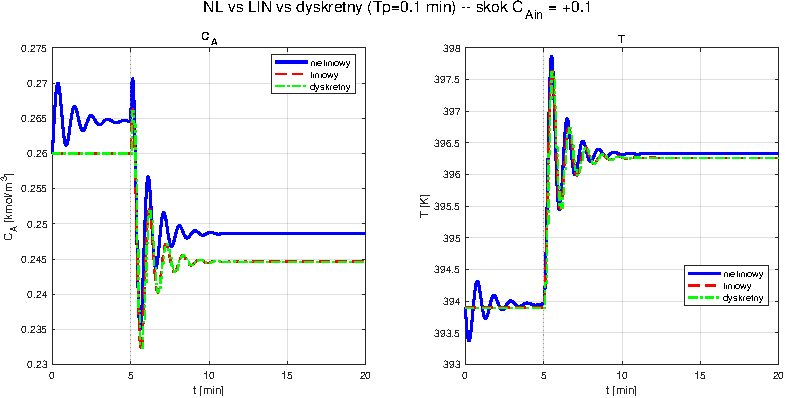
\includegraphics[width=0.95\textwidth]{wykresy/1d_weryfikacja_CAin.pdf}
    \caption{Porównanie NL vs LIN ciągły vs dyskretny -- skok $\Delta C_{Ain} = +0{,}1$}
    \label{fig:1d_werf_cain}
\end{figure}

\begin{figure}[H]
    \centering
    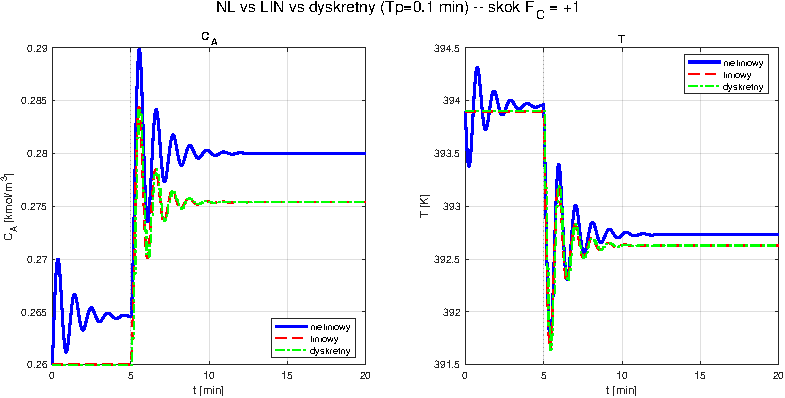
\includegraphics[width=0.95\textwidth]{wykresy/1d_weryfikacja_FC.pdf}
    \caption{Porównanie NL vs LIN ciągły vs dyskretny -- skok $\Delta F_C = +1$}
    \label{fig:1d_werf_fc}
\end{figure}

Dla małych skoków wszystkie trzy krzywe praktycznie się pokrywają, co potwierdza poprawność dyskretyzacji -- model dyskretny wiernie odwzorowuje model liniowy ciągły przy wybranym $T_p = 0{,}1$ min, a~ewentualne różnice względem modelu nieliniowego wynikają wyłącznie z~błędu linearyzacji, nie z~samej dyskretyzacji.

% ==============================================================
\section{Podsumowanie}
% ==============================================================

W~ramach pierwszej części projektu:

\begin{enumerate}
    \item Zaimplementowano i~zasymulowano model nieliniowy reaktora CSTR w~MATLABie.
    \item Wyznaczono model zlinearyzowany w~punkcie pracy -- w~postaci równań stanu oraz transmitancji operatorowych $G(s)$.
    \item Porównano modele liniowy i~nieliniowy dla sekwencji skoków o~różnych amplitudach, wykazując dobrą zgodność dla małych odchyleń.
    \item Ilościowo oceniono jakość aproksymacji -- błąd rośnie z~amplitudą skoku, $T_{in}$ jest najmniej wrażliwe, a~temperatura $T$ jest bardziej podatna na błędy niż stężenie $C_A$.
    \item Opracowano modele dyskretne dla różnych $T_p$, wybierając $T_p = 0{,}1$ min. Zweryfikowano poprawność porównując z~modelem nieliniowym.
\end{enumerate}

\end{document}
